\section{Theorie}
\label{sec:Theorie}
\subsection{Elektrische Leitfähigkeit}
Ein elektrischen Leiter besteht aus einer kristallinen Struktur, in welchem die Valenzelektronen der Atome
ein großes System bilden. Das hat zur Folge, dass sie dem Pauli-Prinzip unterliegen. Demnach muss jedes 
Valenzelektron einen anderen Quantenzustand besitzen. Es gibt nun so viele Elektronen verschiedener Energien,
dass man von quasikontinuierlichen Energiebändern spricht, in denen es jedoch verbotene Zonen gibt.\\
Wie auch in der Versuchsanleitung \cite{AP01}
wird nun ein Na-Atom betrachtet, welches vollständig gefüllte 1s-, 2s-, 2p-Orbitale und ein 3s-Orbital besitzt,
in welchem sich nur ein Elektron befindet. Diese Konfiguration ist in Abbildung \ref{fig:Energiebander}
veranschaulicht. In den gefüllten Orbitalen kann weder Energie aufgenommen noch abgegeben werden. Nur in dem
3s-Orbital ist noch Platz für ein weiteres Elektron.\\
%
\begin{figure}[H]
    \centering
    \includegraphics[scale = 0.3]{content/1Energiebänder.png}
    \caption{Getrennte Energiebänder eines Natriumatoms mit schraffiertem Füllungsgrad in einem Kristall. Quelle: \cite{AP01}}
    \label{fig:Energiebander}
\end{figure}
%
\noindent Wird nun ein elektrisches Feld an das Metall angelegt, können sich Elektronen durch diese Orbitale in Richtung des 
elektischen Feldes bewegen. So entsteht durch die Bewegung der Elektronen aus dem obersten Energieband
ein elektrischer Strom. Dieses oberste Energieband wird deswegen auch Leitfähigkeitsband genannt und die 
Elektronen dieses Bandes Leitungselektronen. Bei nicht leitenden Stoffen befinden sich keine Elektronen in dem
obersten Energieband. Die Leitfähigkeit hängt dabei von Unregelmäßigkeiten in den Kristallen ab.
\subsection{Mathematische Beschreibung der Leitfähigkeit}
Die Bewegung der Leitungselektronen ähnelt der von den Atomen in einem Idealen Gas und kann somit auch ähnlich
berechnet werden. Die Elektronen bewegen sich durch den Leiter und führen dabei Stöße mit Strukturdefekten in 
dem Kristallgitter.\\\\
Die mittlere Flugzeit $\bar{\tau}$ beschreibt nun die durchschnittliche Zeit zwischen zwei Stößen des Elektrons mit
dem Gitter. Während dieser Zeit wird ein Elektron in einem elektischen Feld gleichmäßig beschleunigt. Diese
Beschleunigung ist dabei
\begin{equation*}
    \vec{b}=-\frac{e_0}{m_0}\vec{E}
\end{equation*}
mit der Ladung $-e_0$ und der Ruhemasse $m_0$ des Elektrons. Die Geschwindigkeitsänderung $\Delta\vec{\bar{v}}$
Während $\bar{\tau}$ ist dann also
\begin{equation*}
    \Delta\vec{\bar{v}}=\vec{b}\bar{\tau}.
\end{equation*}
Nach jedem Stoß wird das Elektron dann zufällig gestreut und wird dann wieder von dem elektischen Feld
beschleunigt. Deswegen führt man die mittlere Driftgeschwindigkeit $\vec{\bar{v}}_d$ ein, für welche 
\begin{equation*}
    \vec{\bar{v}}_d=\frac{1}{2}\Delta\vec{\bar{v}}
\end{equation*}
gilt. \\\\
Nun kann über die mittlere Driftgeschwindigkeit die Stromdichte $\vec{j}$ definiert werden. Diese gibt an
wie viele Elektronen durch einen Leiter mit bestimmtem Querschnitt fließen. Die Stromdichte ist dabei durch
\begin{equation}
    \vec{j}=-n \vec{\bar{v}}_d e_0
    =\frac{1}{2}\frac{e_0^2}{m_0}n\bar{\tau}\vec{E} \label{eqn:j}
\end{equation}
definiert, wobei $n$ die Anzahl der Elektronen ist. Bei einem homogenen Leiter mit Länge $L$ und Querschnitt
$Q$ gilt zudem
\begin{align*}
    j=\frac{I}{Q} \qquad \text{und} \qquad E=\frac{U}{L}.
\end{align*}
Einsetzen in Gleichung \eqref{eqn:j} liefert
\begin{equation}
    I=\frac{1}{2}\frac{e_0^2}{m_0}n\bar{\tau}\frac{Q}{L}U. \label{eqn:I}
\end{equation}
Definiert man nun die Leitfähigkeit $S$ durch
\begin{equation*}
    S=\frac{1}{2}\frac{e_0^2}{m_0}n\bar{\tau}\frac{Q}{L}
\end{equation*}
fällt auf, dass \eqref{eqn:I} die Form des Ohmschen Gesetztes besitzt
\begin{equation*}
    U=S\cdot U, \qquad \text{mit}\quad S=\frac{1}{R}.
\end{equation*}
Der Widerstand $R$ ist also gegeben durch
\begin{equation}
    R=2\frac{m_0}{e_0^2}\frac{1}{n\bar{\tau}}\frac{L}{Q}. \label{eqn:R}
\end{equation}
%Vielleicht braucht man das hier gar nicht
Nun kann durch den Widerstand $R$ und die Leitfähigkeit $S$ der spezifische Widerstand $\rho$ und
die spezifische Leitfähigkeit $\sigma$ berechnet werden. Dies erfolgt durch
\begin{equation*}
    \sigma=\frac{1}{2}\frac{e_0^2}{m_0}n\bar{\tau} 
    \quad \text{und} \quad
    \rho=2\frac{m_0}{e_0^2}\frac{1}{n\bar{\tau}}.
\end{equation*}
%Bis hier
Der Widerstand $R$ ist nun eine präzise messbare Größe, über welche mit Gleichung \ref{eqn:R} Aussagen
über die Bewegung der Elektronen im Leiter getroffen werden können. Jedoch müssen noch die unbekannten
Größen $n$ und $\bar{\tau}$ näher beleuchtet werden.
\subsection{Der Hall-Effekt}
Der Hall-Effekt tritt auf, wenn eine stromdurchflossene Leiterplatte senkrecht in ein Magnetfeld 
gebracht wird. Durch die Lorenzkraft $F_L$ werden die Elektronen gemäß der 3-Finger-Regel auf der Leiterplatte
verschoben. Der Betrag der Lorenzkraft ist dabei gegeben durch
\begin{equation*}
    F_L=e_0\bar{v}B.
\end{equation*} 
Dadurch entsteht eine Potentialdifferenz auf der Leiterplatte. Diese Potentialdifferenz wird 
Hall-Spannung genannt. \\
In Abbildung \ref{fig:Hall} ist die beschriebne Versuchsanordnung noch einmal visualisiert.
Die Elektronen bewegen sich dabei in negative x-Richtung, der magnetische Fluss verläuft in positive z-Richtung.
Nach der 3-Finger-Regel (linke Hand für negative Ladungen) wird schnell ersichtlich, dass die Lorenzkraft die 
Elektronen in negative y-Richtung verschiebt.
%
\begin{figure}[H]
    \centering
    \caption{Versuchsaufbau zur Messung der Hallspannung. Quelle: \cite{AP01}}
    \label{fig:Hall}
      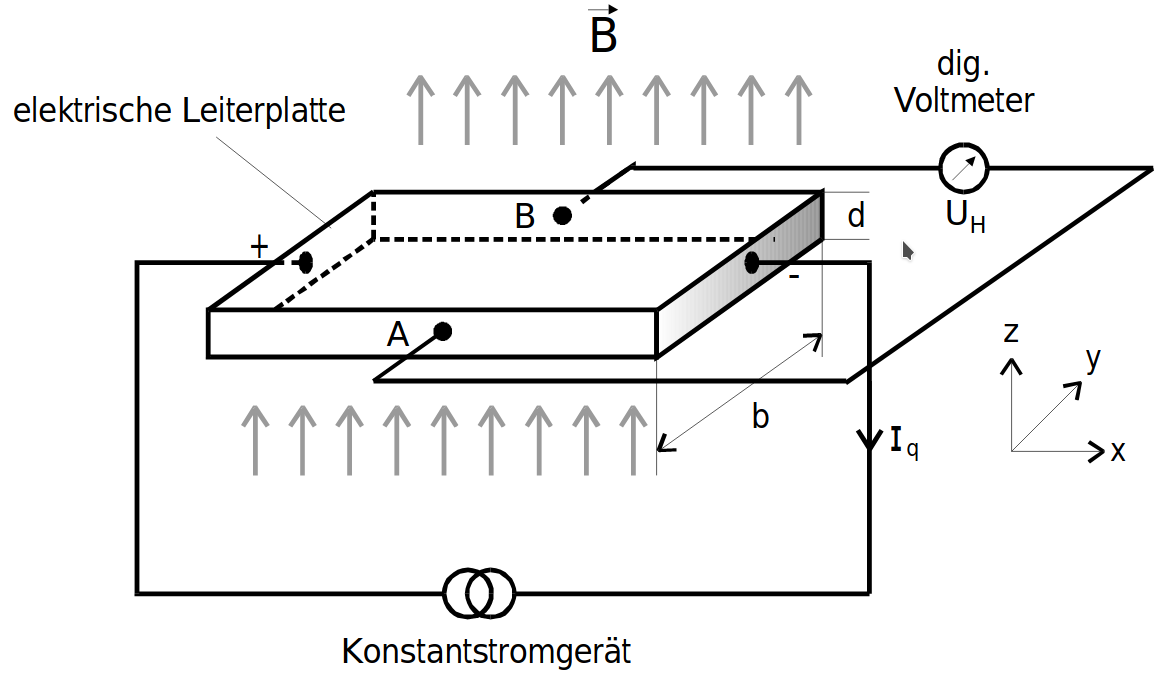
\includegraphics[scale = 0.3]{content/1Hall.png}
  \end{figure}
%
\noindent Die Hallspannung $U_H$ ist dabei durch
\begin{equation}
    U_H=\bar{v}_dB\cdot b \label{eqn:Uh1}
\end{equation}
gegeben, wobei man $\bar{v_d}$ schreiben kann als 
\begin{equation}
    \bar{v_d}=-\frac{1}{ne_0}\frac{I_q}{bd}. \label{eqn:vd}
\end{equation}
Dabei ist $b$ die Breite und $d$ die Dicke der Leiterplatte wie auch in Abbildung \ref{fig:Hall} zu erkennen.
Dadurch lässt sich Gleichung \eqref{eqn:Uh1} schreiben als 
\begin{equation}
    U_H=-\frac{1}{ne_0}\frac{B\cdot I_q}{d}. \label{eqn:Uh2}
\end{equation}
Die Größen $U_h$, $B$, $I_d$, $b$ und $d$ sind nun ohne viel Aufwand zu messen. Somit kann dann durch 
Gleichung \ref{eqn:Uh2} $n$ und durch Gleichung \ref{eqn:vd} $v_d$ bestimmt werden. Da $n$ nun bekannt ist,
kann durch Gleichung \ref{eqn:R} nach der Messung von $R$ auch $\tau$ berechnet werden.\\
\subsection{Weitere Leitfähigkeitsparameter}
Aus den errechneten Parametern lassen sich nun noch weitere Parameter ableiten, die weitere Informationen 
über die Bewegung der Elektronen liefern.\\\\
Interessant ist die mittlere freie Weglänge $\bar{l}$, die die Elektronen in der Zeit $\bar{\tau}$ zurücklegen, bevor
sie wieder mit dem Gitter stoßen. $\bar{l}$ kann dabei durch
\begin{equation*}
    \bar{l}=\bar{\tau}\cdot v_T
\end{equation*}
berechnet werden. $v_T$ ist dabei die Totalgeschwindigkeit des Elektrons, welche durch die Brownsche Bewegung 
%vielleicht besser Wärmebewegung?
der Kristallbausteine erzeugt wird.\\
Versteht man die Leitungselektronen wie Atome in einem Idealen Gas, so besitzt ein Elektron die kinetische Energie
\begin{equation}
    E_{kin}=\frac{3}{2}kT=\frac{1}{2}m_0v_T^2 . \label{eqn:Ekin}
\end{equation}
Dabei entspricht $k$ der Bolzmann Konstante. Umstellen von \eqref{eqn:Ekin} liefert
\begin{equation}
    v_T=\sqrt{\frac{3kT}{m_0}}. \label{eqn:vT1}
\end{equation}
Allerdings muss bei den Elektronen das Anfangs erwähnte Pauli-Prinzip beachtet werden. So muss die Fermi-Dirac-Verteilung
\begin{equation*}
    f(E)dE=\frac{1}{e^{\frac{E-E_f}{kT}}+1}dE
\end{equation*}
verwendet werden, um zu beschreiben, wie Groß die Wahrscheinlichkeit $f(E)$ ist, ein 
Elektron mit der Engerie bis $E+dE$ anzutreffen. $E_F$ ist dabei die Fermi-Energie, die durch
\begin{equation}
    E_F=\frac{h^2}{2m_0}\sqrt[3]{\left(\frac{3n}{8\pi}\right)^2} \label{eqn:EF}
\end{equation}
gegeben ist. $h$ ist hierbei das Plancksche Wirkungsquantum. \\\\
\eqref{eqn:EF} ist nun sehr viel besser geeignet um $v_T$ zu bestimmen als \ref{eqn:Ekin}. 
Für die Leitungselektronen kann nun $E \approx E_F$ aufgenommen werden.
$v_T$ kann dann beschrieben werden als
\begin{equation*}
    v_T\approx\sqrt{\frac{2E_F}{m_0}}.
\end{equation*}
Dadruch folgt für die mittlere freie Weglänge $\bar{l}$
\begin{equation*}
    \bar{l}\approx\bar{\tau}\sqrt{\frac{2E_F}{m_0}}.
\end{equation*}
Nun kann noch die Beweglichkeit $\mu$ der Elektronen bestimmt werden. Diese ist genau der Faktor, der 
das elektrische Feld mit der Driftgeschwindigkeit verbindet. Es gilt
\begin{equation*}
    \vec{\bar{v}}_d=\mu \vec{E}.
\end{equation*}
\section{Der anormale Hall-Effekt}
Es kann vorkommen, dass sich Energiebänder überlappen und Elektronen dann von dem unteren in das höhere Band
springen. Dadurch entstehen sogenannte Löcher in den Bändern, die sich wie positive Ladungen verhalten, sich 
in einem elektrischen Feld also in die umgekehrte Richtung wie die Elektronen bewegen. Dies wird anormaler 
Hall-Effekt genannt.